% !TeX spellcheck = cs_CZ
%{\tikzset{external/prefix={tikz/FYZII/}}
% \tikzset{external/figure name/.add={ch28_}{}}
%---------------------------------------------------------------------------------------------------
% file fey2ch28.tex
%---------------------------------------------------------------------------------------------------
%=========================== Kapitola Elektromagnetická hmotnost ===================================
\setchaptertoc
\chapter{Elektromagnetická hmotnost}\label{fyz:IIchapXXIIX}

  \section{Energie pole bodového náboje}\label{fyz:IIchapXXIIXsecI}
  \section{Hybnost pole pohybujícího se náboje}\label{fyz:IIchapXXIIXsecII}
  \section{Elektromagnetická hmotnost}\label{fyz:IIchapXXIIXsecIII}
  \section{Síla, kterou elektron působí sám na sebe}\label{fyz:IIchapXXIIXsecIV}
  \section{Pokusy o modifikaci Maxwellovy teorie}\label{fyz:IIchapXXIIXsecV}
  \section{Pole jaderných sil}\label{fyz:IIchapXXIIXsecVI}
  \section{Příklady a cvičení}\label{fyz:IIchapXXIIXsecVII}

    \begin{figure}[ht!] %\ref{fyz:fig617}
      \centering
      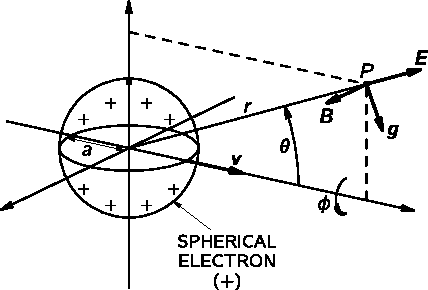
\includegraphics[width=0.7\linewidth]{fyz_fig617.pdf}
      \caption{
               (\cite[s.~707]{Feynman02})}
      \label{fyz:fig617}
    \end{figure}

    \begin{figure}[ht!] %\ref{fyz:fig618}
      \centering
      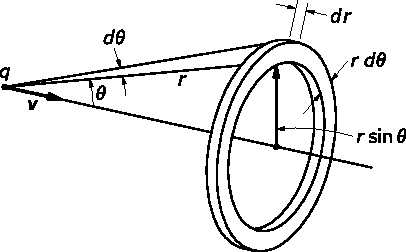
\includegraphics[width=0.7\linewidth]{fyz_fig618.pdf}
      \caption{
               (\cite[s.~707]{Feynman02})}
      \label{fyz:fig618}
    \end{figure}

    \begin{figure}[ht!]
      \centering
      \subcaptionbox{\label{fyz:fig619a}}{\luafigure[0.3]{fyz_fig619a.pdf}}
      \subcaptionbox{\label{fyz:fig619b}}{\luafigure[0.3]{fyz_fig619b.pdf}}
      \subcaptionbox{\label{fyz:fig619c}}{\luafigure[0.3]{fyz_fig619c.pdf}}
      \label{fyz:fig619}
      \caption{
               (\cite[s.~748]{Feynman02})}
    \end{figure}

    \begin{figure}[ht!] %\ref{fyz:fig620}
      \centering
      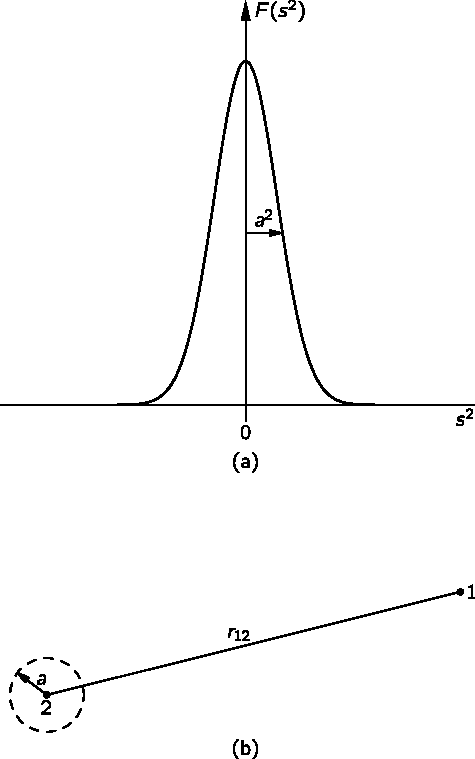
\includegraphics[width=0.7\linewidth]{fyz_fig620.pdf}
      \caption{
               (\cite[s.~707]{Feynman02})}
      \label{fyz:fig620}
    \end{figure}

    \begin{figure}[ht!] %\ref{fyz:fig621}
      \centering
      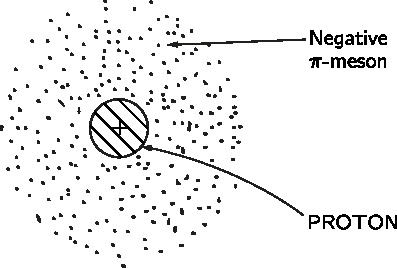
\includegraphics[width=0.7\linewidth]{fyz_fig621.pdf}
      \caption{
               (\cite[s.~707]{Feynman02})}
      \label{fyz:fig621}
    \end{figure}

    \begin{figure}[ht!] %\ref{fyz:fig622}
      \centering
      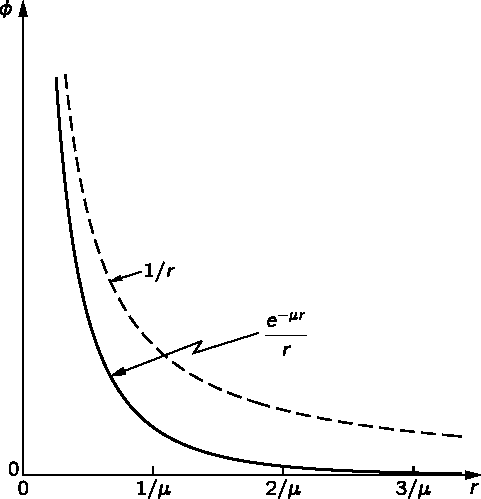
\includegraphics[width=0.7\linewidth]{fyz_fig622.pdf}
      \caption{
               (\cite[s.~707]{Feynman02})}
      \label{fyz:fig622}
    \end{figure}

    \todo[inline]{Kapitola fey2ch28 je nedodělaná, obsahuje pouze obrázky}
%} %tikzset
%---------------------------------------------------------------------------------------------------
